


\section{Conditions : Si, alors, sinon}
\begin{UPSTIinfor}{Qu'est-ce qu'une condition ?}
    \vspace{1em}
\textbf{Une condition est une instruction qui permet de prendre des décisions dans un programme.}\\\\
Par exemple, si l'utilisateur a plus de 18 ans, on peut lui afficher un message différent que s'il a moins de 18 ans.
\end{UPSTIinfor}

Sur Scratch, on utilise le bloc "si [condition] alors" pour créer une condition. 
On peut aussi utiliser le bloc "sinon" pour exécuter un bloc de code si la condition n'est pas remplie.

\subsection{Conditions simples}
\begin{UPSTIManipulation}{Condition simple}
\begin{itemize}[label=$\square$]
        \item Demander à l'utilisateur son âge et stocker la réponse dans une variable "Âge".
        \item Utiliser un bloc "si [Âge > 18] alors"
        \item Dans le bloc "si", ajouter un bloc "dire [Vous êtes majeur]" pour afficher un message si l'utilisateur est majeur.
        \item Ajouter un bloc "sinon" pour afficher un message différent si l'utilisateur est mineur.
        \item Cliquez sur le drapeau vert pour exécuter votre programme. Vous devriez voir le sprite demander votre âge et afficher un message différent selon que vous êtes majeur ou mineur.
        \end{itemize}
\end{UPSTIManipulation}

\subsection{Conditions imbriquées}
Les conditions peuvent aussi être imbriquées, c'est-à-dire qu'on peut mettre une condition à l'intérieur d'une autre condition. 

\begin{UPSTIManipulation}{Condition imbriquée}
    \begin{itemize}[label=$\square$]
        \item Créer un programme qui dit à l'utilisateur s'il est un enfant (0-12 ans), un adolescent (13-17 ans), un adulte (18-64 ans) ou un senior (65 ans et plus).
        \item Pour cela, vous devrez utiliser des conditions imbriquées.
        \item Faire valider votre programme par l'enseignant.
    \end{itemize}
    \begin{minipage}{.5\textwidth}
        \begin{center}
            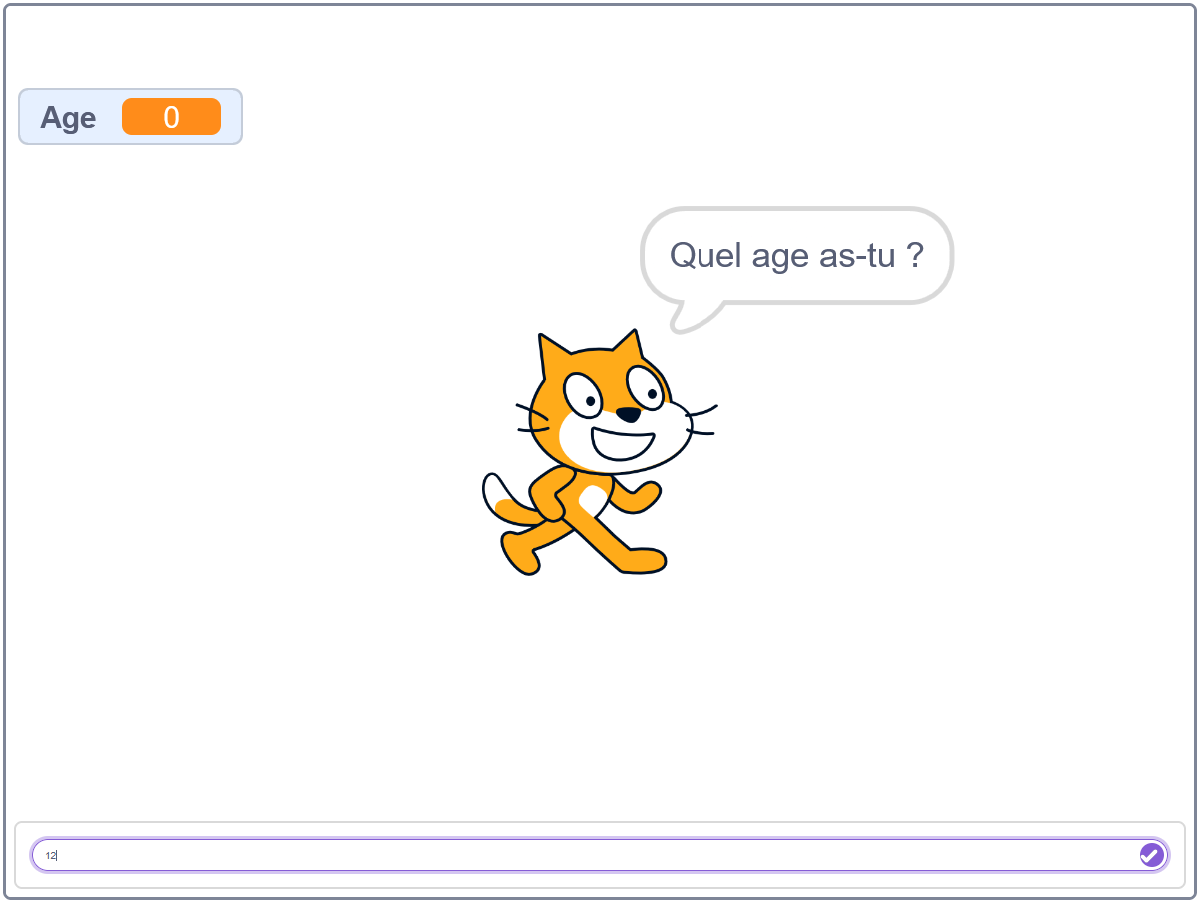
\includegraphics[width=.9\linewidth]{age.png}
        \end{center}
    \end{minipage}\hfill
    \begin{minipage}{.5\textwidth}
        \begin{center}
            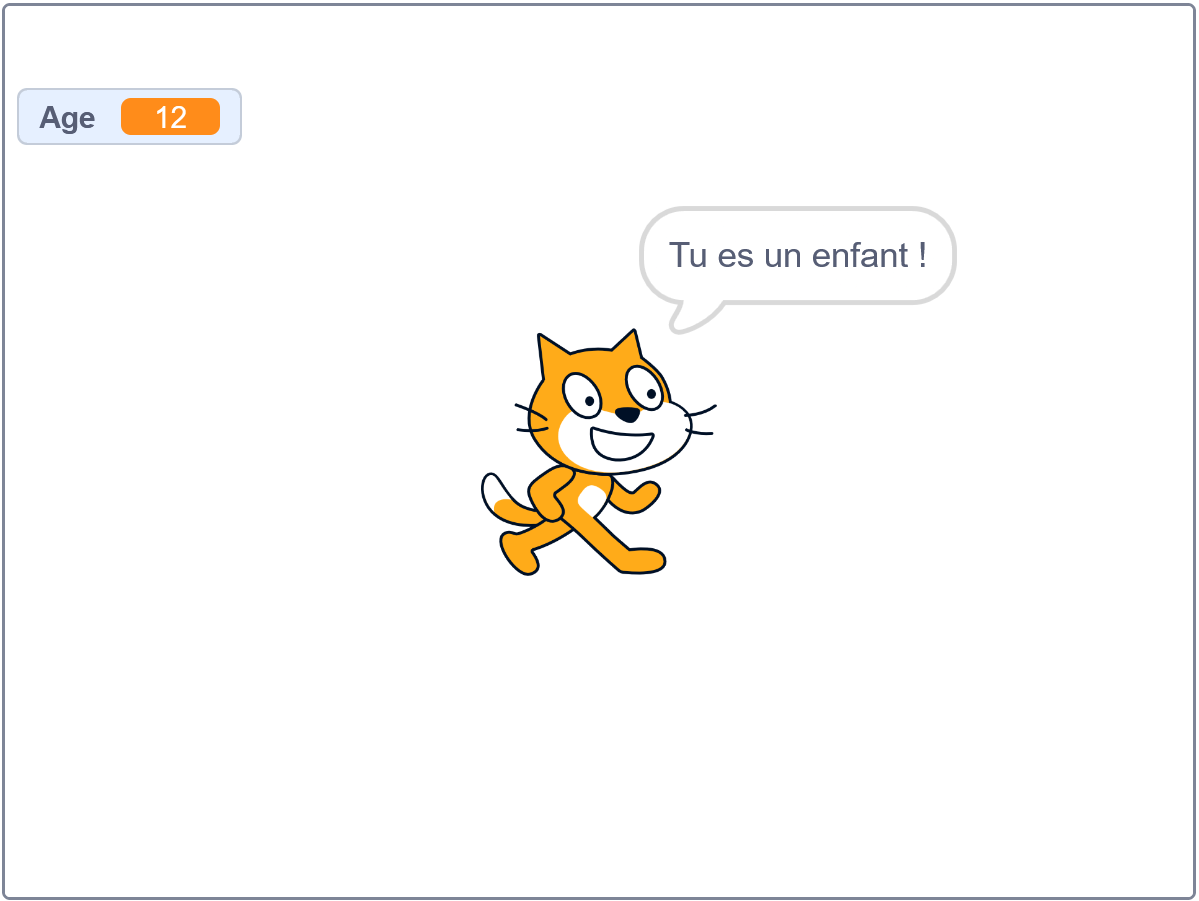
\includegraphics[width=.9\linewidth]{age-reponse.png}
        \end{center}
    \end{minipage}
\end{UPSTIManipulation}